\documentclass{beamer}
\usetheme{Berlin}
\usepackage[T1]{fontenc}
\usepackage{minted}
\usepackage{etoolbox}
\usepackage{setspace}
\usepackage{bussproofs}
\usepackage{amsmath}
\usepackage{amsthm}
\usepackage{amssymb}

\BeforeBeginEnvironment{minted}{\begin{spacing}{1.0}}
\AfterEndEnvironment{minted}{\end{spacing}}
\AfterEndEnvironment{minted}{\vspace{0pt}}

\DeclareUnicodeCharacter{22A8}{\(\vDash\)}
\DeclareUnicodeCharacter{22A2}{\(\vdash\)}
\DeclareUnicodeCharacter{2286}{\(\subseteq\)}
\DeclareUnicodeCharacter{22AB}{\(\VDash\)}
\DeclareUnicodeCharacter{2291}{\(\sqsubseteq\)}
\DeclareUnicodeCharacter{03A3}{\(\Sigma\)}
\DeclareUnicodeCharacter{03C1}{\(\rho\)}

\title{Primjene Coq alata za dokazivanje u matematici i računarstvu}
\subtitle{Logika prvog reda s induktivnim definicijama}
\author{Miho Hren}
\institute{Mentori: Vedran Čačić, Marko Doko \(+\) Ante Đerek\\
  Fakultet Elektrotehnike i Računarstva}
\date{2023./2024.}

\setbeamertemplate{headline}{}
\setbeamertemplate{footline}[frame number]
\setbeamertemplate{navigation symbols}{}


\begin{document}
\begin{frame}
  \titlepage{}
\end{frame}

\begin{frame}
  \frametitle{Proces}
  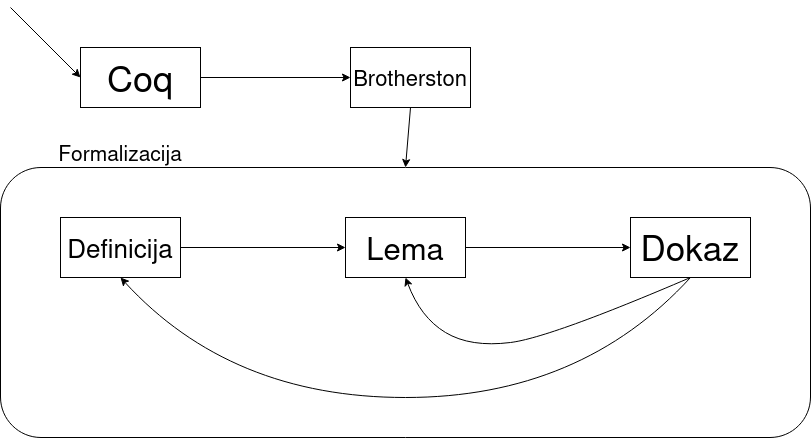
\includegraphics[width=\textwidth]{diplomskiproces.png}
\end{frame}

\begin{frame}[fragile]
  \frametitle{Sintaksa: signatura}
\begin{minted}{coq}
Structure signature := {
    FuncS : Set;
    fun_ar : FuncS -> nat;
    PredS : Set;
    pred_ar : PredS -> nat;
    IndPredS : Set;
    indpred_ar : IndPredS -> nat;
  }.
\end{minted}
  \begin{block}{Peanova signatura}
      \[
    \sigma_{\mathit{PA}} = \{ \{ o^{0}, s^{1}, +^{2}, \cdot^{2} \},
    \{=^{2}\}, \{\mathit{Nat}^{1}, \mathit{Even}^{1}, \mathit{Odd}^{1}\}\}
  \]
  \end{block}
\end{frame}

\begin{frame}[fragile]
  \frametitle{Sintaksa: termi, formule}
\begin{minted}{coq}
Inductive term  : Set :=
| var_term : var -> term 
| TFunc : forall (f : FuncS Σ),
    vec term (fun_ar f) -> term.

Inductive formula : Set :=
| FPred (P : PredS Σ)
    : vec (term Σ) (pred_ar P) -> formula 
| FIndPred (P : IndPredS Σ)
    : vec (term Σ) (indpred_ar P) -> formula 
| FNeg : formula -> formula 
| FImp : formula -> formula -> formula 
| FAll : formula -> formula.
\end{minted}

\end{frame}

\begin{frame}[fragile]
  \frametitle{Sintaksa: produkcije}
  \begin{huge}
    \begin{prooftree}
      \AxiomC{\(  Q_{1}\mathbf{u}_{1}  \ldots   Q_{n}\mathbf{u}_{n}  \)}
      \AxiomC{\(  P_{1}\mathbf{v}_{1}  \ldots   P_{m}\mathbf{v}_{m}  \)}
      \BinaryInfC{\(P\mathbf{t}\)}
    \end{prooftree}
  \end{huge}
  \begin{small}
\begin{minted}{coq}
Record production :=
  mkProd {
      preds
        : list {P: PredS Σ & vec (term Σ) (pred_ar P)};
      indpreds
        : list {P: IndPredS Σ & vec (term Σ) (indpred_ar P)};
      indcons : IndPredS Σ;
      indargs : vec (term Σ) (indpred_ar indcons);
    }.
\end{minted}
  \end{small}
\end{frame}

\begin{frame}
  \begin{block}{Biti prirodan broj.}
    \begin{minipage}[t]{0.48\linewidth}
      \begin{prooftree}
        \AxiomC{}
        % \RightLabel{(\texttt{PA\_prod\_N\_zero})}
        \UnaryInfC{\( \mathit{Nat}(o) \)}
      \end{prooftree}
    \end{minipage}
    \begin{minipage}[t]{0.48\linewidth}
      \begin{prooftree}
        \AxiomC{\( \mathit{Nat}(x) \)}
        % \RightLabel{(\texttt{PA\_prod\_N\_succ})}
        \UnaryInfC{\( \mathit{Nat}(s(x)) \)}
      \end{prooftree}
    \end{minipage}
  \end{block}
  \begin{block}{Biti paran, odnosno neparan broj.}
    \begin{minipage}[t]{0.31\linewidth}
      \begin{prooftree}
        \AxiomC{}
        % \RightLabel{(\texttt{PA\_prod\_E\_zero})}
        \UnaryInfC{\( \mathit{Even}(o) \)}
      \end{prooftree}
    \end{minipage}
    \begin{minipage}[t]{0.31\linewidth}
      \begin{prooftree}
        \AxiomC{\( \mathit{Odd}(x) \)}
        % \RightLabel{(\texttt{PA\_prod\_E\_succ})}
        \UnaryInfC{\( \mathit{Even}(s(x)) \)}
      \end{prooftree}
    \end{minipage}
    \begin{minipage}[t]{0.31\linewidth}
      \begin{prooftree}
        \AxiomC{\( \mathit{Even}(x) \)}
        % \RightLabel{(\texttt{PA\_prod\_O\_succ})}
        \UnaryInfC{\( \mathit{Odd}(s(x)) \)}
      \end{prooftree}
    \end{minipage}
  \end{block}
\end{frame}

\begin{frame}[fragile]
  \frametitle{Semantika: struktura, okolina}
\begin{minted}{coq}
Structure structure := {
    domain :> Set;
    interpF (f : FuncS Σ)
        : vec domain (fun_ar f) -> domain;
    interpP (P : PredS Σ)
        : vec domain (pred_ar P) -> Prop;
    interpIP (P : IndPredS Σ)
        : vec domain (indpred_ar P) -> Prop;
  }.

Definition env := var -> M.
\end{minted}
  \begin{block}{Standardna Peanova struktura}
    \[
      M_{\mathit{PA}} = (\mathbb{N}, 0, S, +, \cdot, =, \mathbb{N}, \mathbb{E}, \mathbb{O})
    \]
  \end{block}
\end{frame}

\begin{frame}[fragile]
  \frametitle{Semantika: istinitost formule}
\begin{minted}{coq}
Fixpoint Sat (ρ : env M) (F : formula Σ) : Prop :=
  match F with
  | FPred P args => interpP P (V.map (eval ρ) args)
  | FIndPred P args => interpIP P (V.map (eval ρ) args)
  | FNeg G => ~ Sat ρ G
  | FImp F G => Sat ρ F -> Sat ρ G
  | FAll G => forall d, Sat (d .: ρ) G
  end.
\end{minted}
  \begin{block}{Primjer}
    \[
      (M_{\mathit{PA}}, \rho) \vDash \forall x, \mathit{Nat}(x) \rightarrow \mathit{Even}(x) \lor \mathit{Odd}(x)
    \]
  \end{block}
\end{frame}

\begin{frame}
  \frametitle{Semantika: produkcije}
  
\end{frame}






\end{document}
%%% Local Variables:
%%% mode: LaTeX
%%% TeX-master: t
%%% End:
